\documentclass[%
  a4paper,%
  11pt,% <10pt, 9pt>
  %style=screen,
  %sender=bottom,
  blue,% <orange, green, violet>
  %rgb, <cmyk>
  %mono,
  hyperref	% tubs color for hyperref
  ]{tubsartcl}
\usepackage[utf8]{inputenc}
\usepackage{hyperref}

\setlength{\parindent}{0cm}
 
% Titelseiten-Elemente
\title{TuringBrain IDE \LARGE 1.0}
\subtitle{User Guide}
\author{\small Vanessa Baier, Nils Breyer, Phillipp Neumann,\\ Sven Schuster, David Wille}
\logo{
\includegraphics{ips}}
\titleabstract{TuringBrain IDE -- User Guide}
\titlepicture{title}
% Rückseiten-Elemente
\address{
  Advisor: Matthias Hagner\\\\
  Technische Universität Braunschweig\\
  Institut für Programmierung und Reaktive Systeme\\
  Mühlenpfordtstr. 23\\
  38106 Braunschweig}
\backpageinfo{
}

\begin{document}

\maketitle[image,logo=right]%[<plain/image/imagetext>,<logo=left/right>]

\tableofcontents
\newpage
\section{Introduction}

TuringBrain IDE allows you to develop and debug your own TuringMachines in an easy to use WYSIWYG (what you see is what you get) environment. It also enables you to program and run Brainfuck code.



\subsection{Features}

\begin{itemize}
  \item Edit Turing Machines by graphically editing the state graph
  \item Create Turing Machines with multiple tapes
  \item Write Brainfuck programs within the integrated code editor
  \item Simulate your machines and programs using the integrated simulation
  \item Simulate on special LEGO-Tape (hardware needed), graphically animated on the screen or on the console
  \item Pause simulation, Debug step-by-step
  \item Live-highlighting of the current state and edge during the simulation
  \item Save machines as .tm (an XML-Format) respective .bf
  \item Copy \& Paste, Undo \& Redo (not yet for Turing Machines)
  \item Export to Latex, SVG, and PNG
  \item and many more features...
\end{itemize}

\section{Getting started}

\subsection{Installation}
\label{sec:installation}

\subsection{Welcome page}
\label{sec:welcome-page}


\section{Turing Machine editor}

\subsection{Edit machine properties}
\label{sec:edit-mach-prop}

\subsection{Adding and changing states}
\label{sec:add-edit-states}

\subsection{Adding and changing edges}
\label{sec:adding-chang-edges}

\subsection{Edit transitions}
\label{sec:edit-transitions}

\subsection{Via points}
\label{sec:via-points}

\subsection{Frames and textboxes}
\label{sec:frames-textboxes}

\subsection{Export}
\label{sec:export}

\section{Brainfuck editor}



\section{Simulation}



\section{Hardware -- LEGO\textregistered\, tape}

This section describes the position of the components used in the machine. The following subsections and pictures are meant to extend the building instructions file created with the LEGO\textregistered\, Digital Designer.

\subsection{The machine's motor section}

Figure \ref{pic:topview} shows a view of the machine's motor section to get a brief overview of it's position and the number 1 -- 4 represent the following pictures.

\begin{figure}[!htb]
\begin{center}
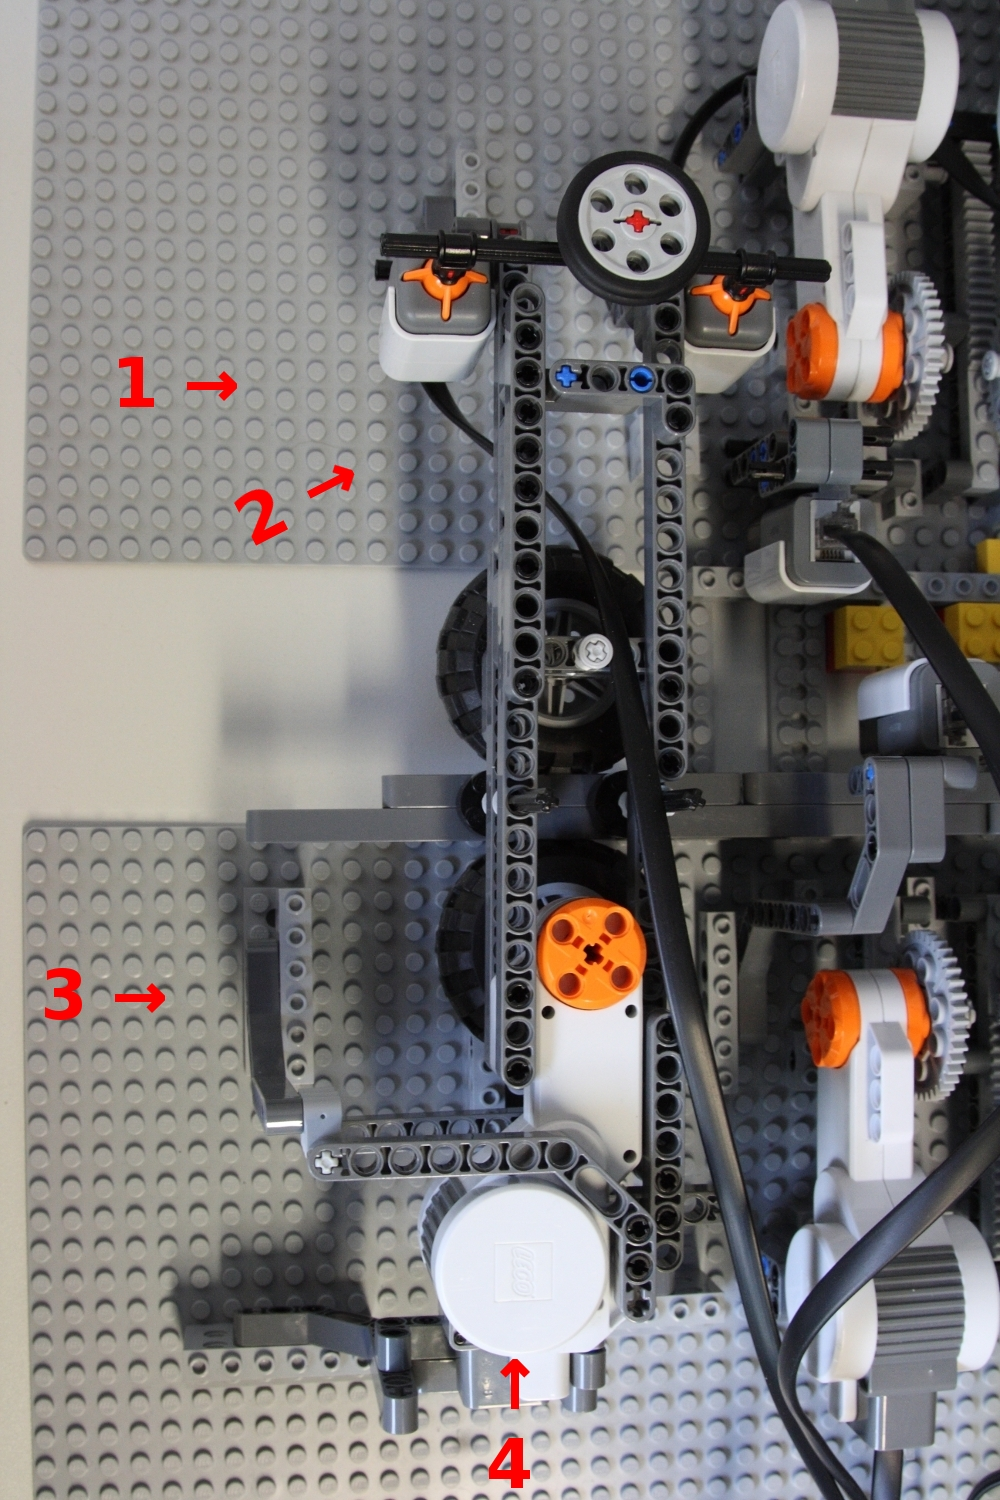
\includegraphics[scale=0.28]{graphics/topview.jpg}
\end{center}
\caption{Overview of the motor section}
\label{pic:topview}
\end{figure}

\newpage

Figure \ref{pic:position1} shows how the upper left pier has to be placed in relation to the left edge of the upper plate.

\begin{figure}[!htb]
\begin{center}
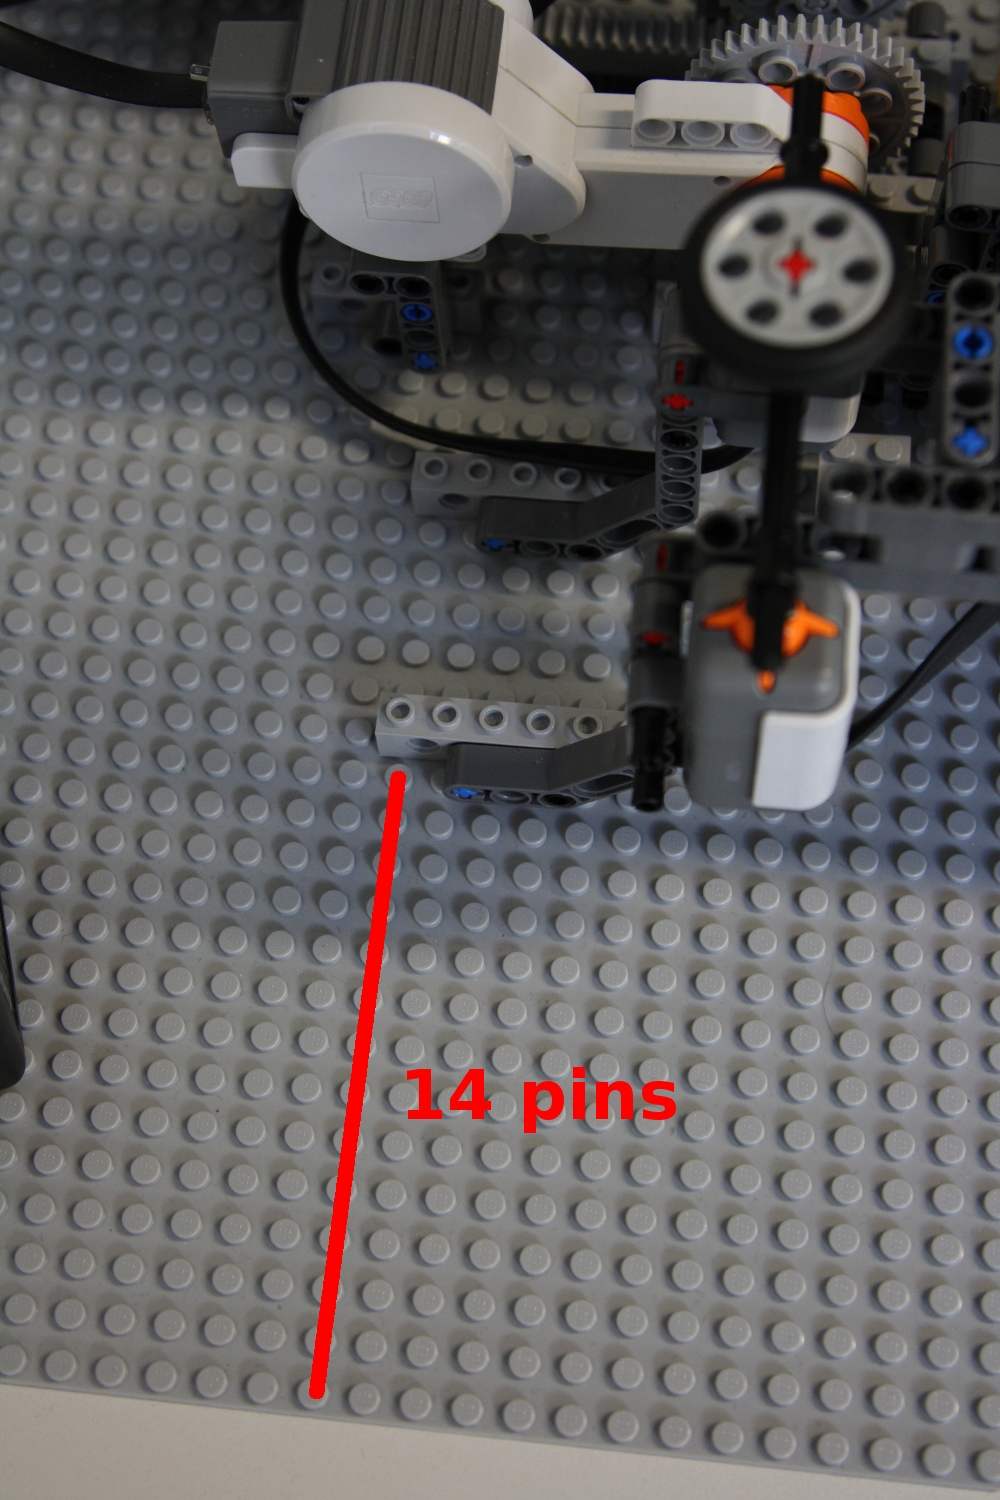
\includegraphics[scale=0.35]{graphics/1.jpg}
\end{center}
\caption{Image taken from position 1}
\label{pic:position1}
\end{figure}

\newpage

Figure \ref{pic:position2} shows how the upper left and right pier have to be placed in relation to the bottom edge of the upper plate.

\begin{figure}[!htb]
\begin{center}
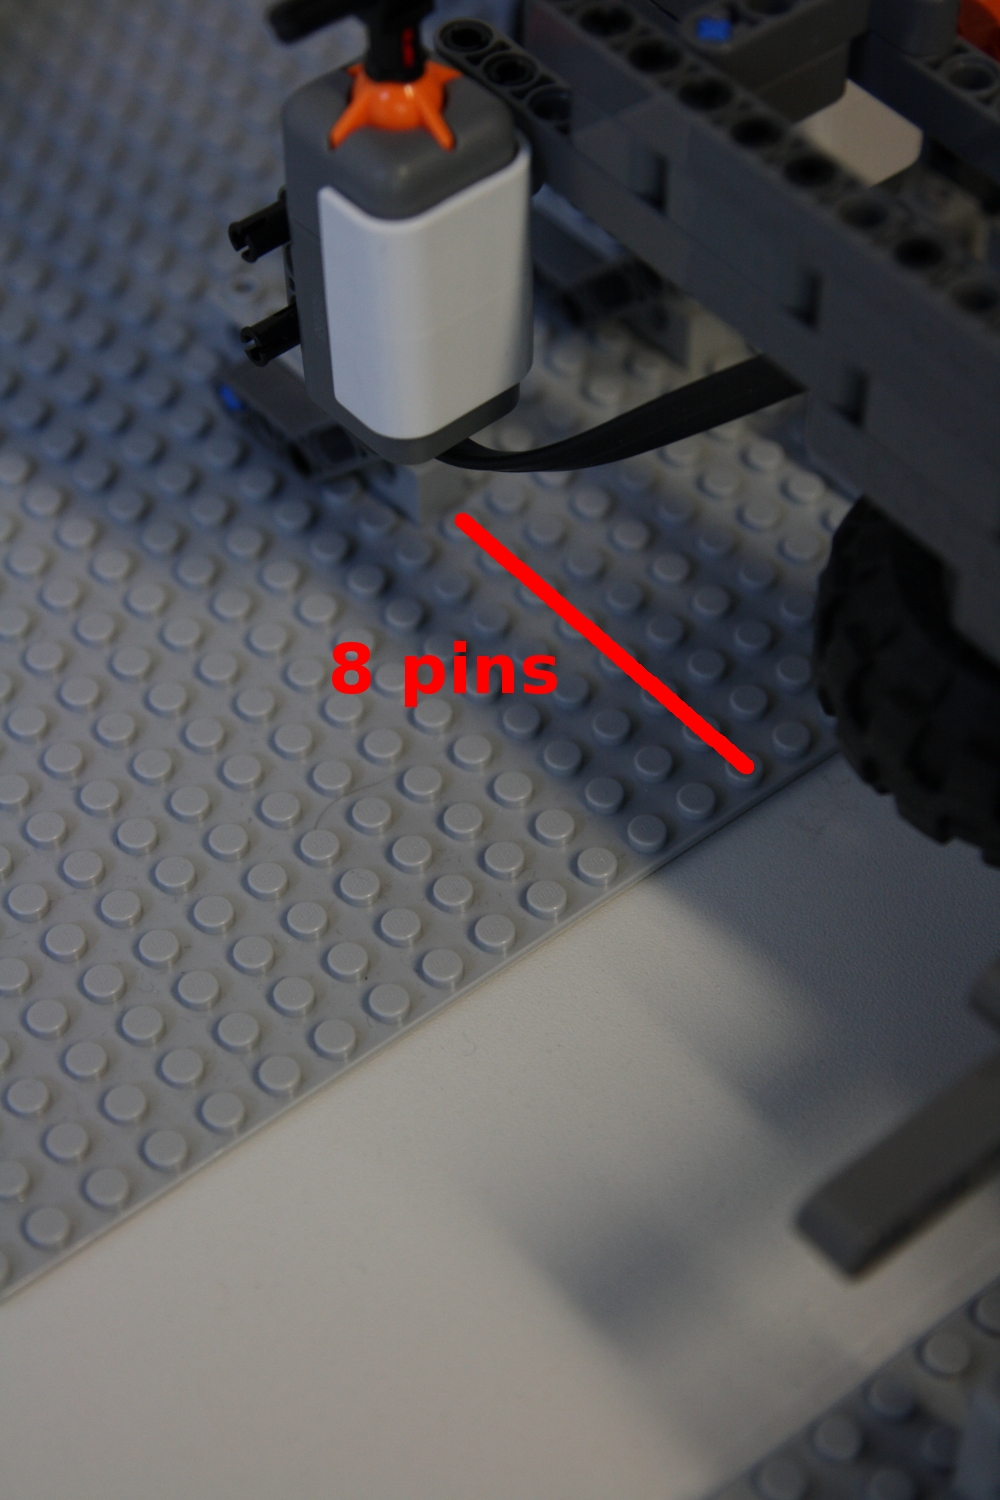
\includegraphics[scale=0.35]{graphics/2.jpg}
\end{center}
\caption{Image taken from position 2}
\label{pic:position2}
\end{figure}

\newpage

Figure \ref{pic:position3} shows how the lower left piers have to be placed in relation to the top and left edge of the lower plate.

\begin{figure}[!htb]
\begin{center}
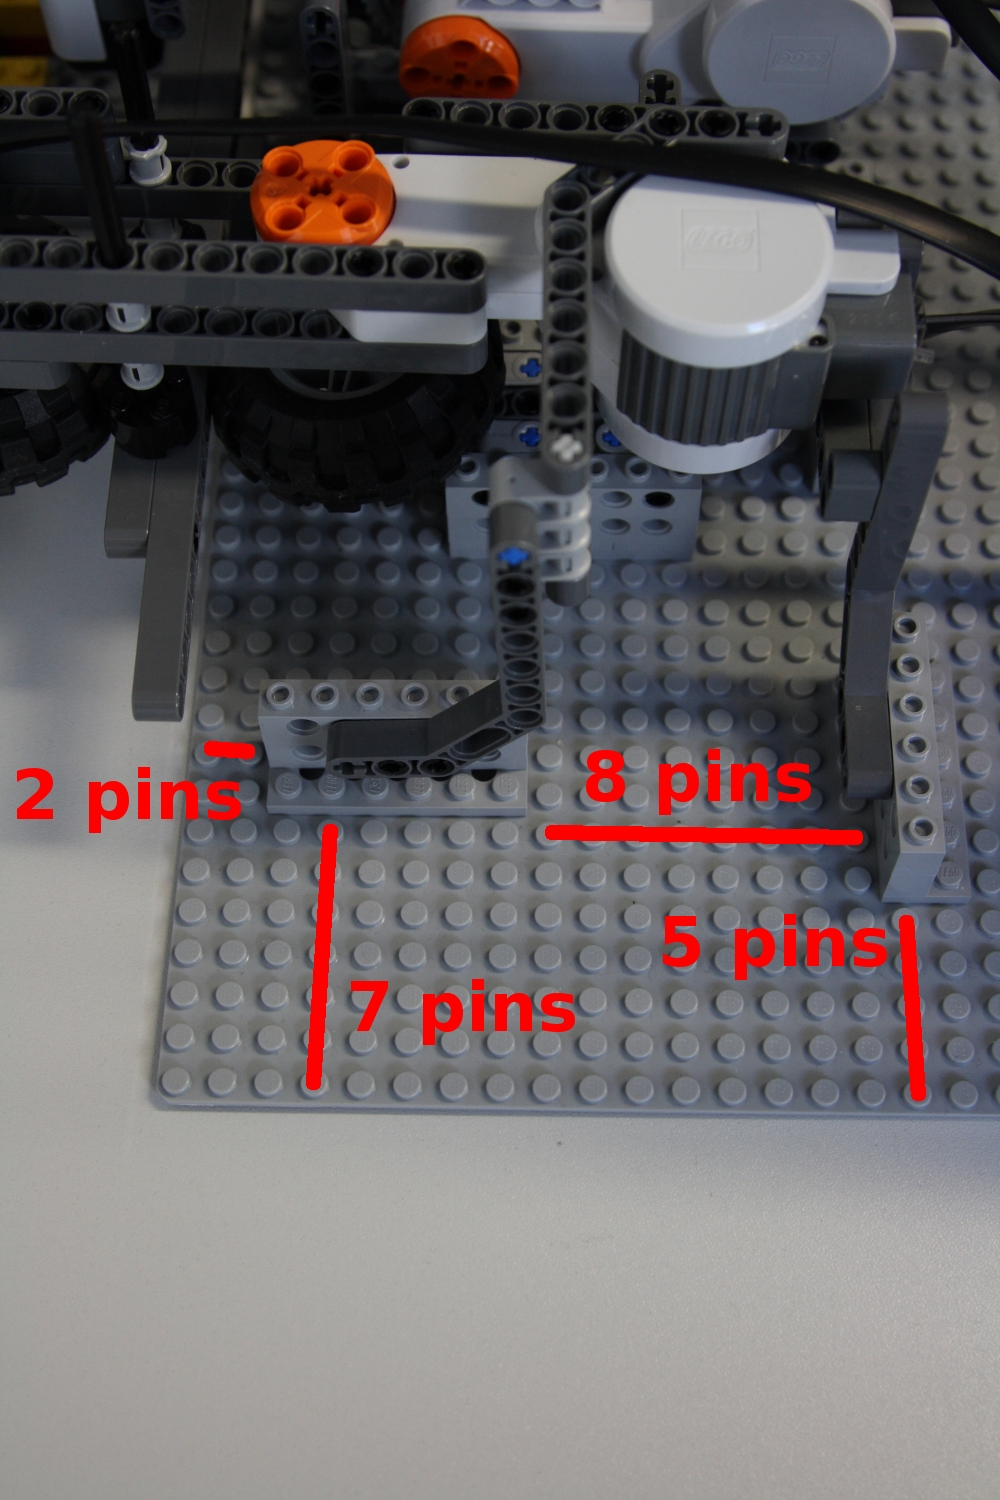
\includegraphics[scale=0.35]{graphics/3.jpg}
\end{center}
\caption{Image taken from position 3}
\label{pic:position3}
\end{figure}

\newpage

Figure \ref{pic:position4} shows how the lower right pier has to be placed in relation to the left pier and the support for the motor wheel.

\begin{figure}[!htb]
\begin{center}
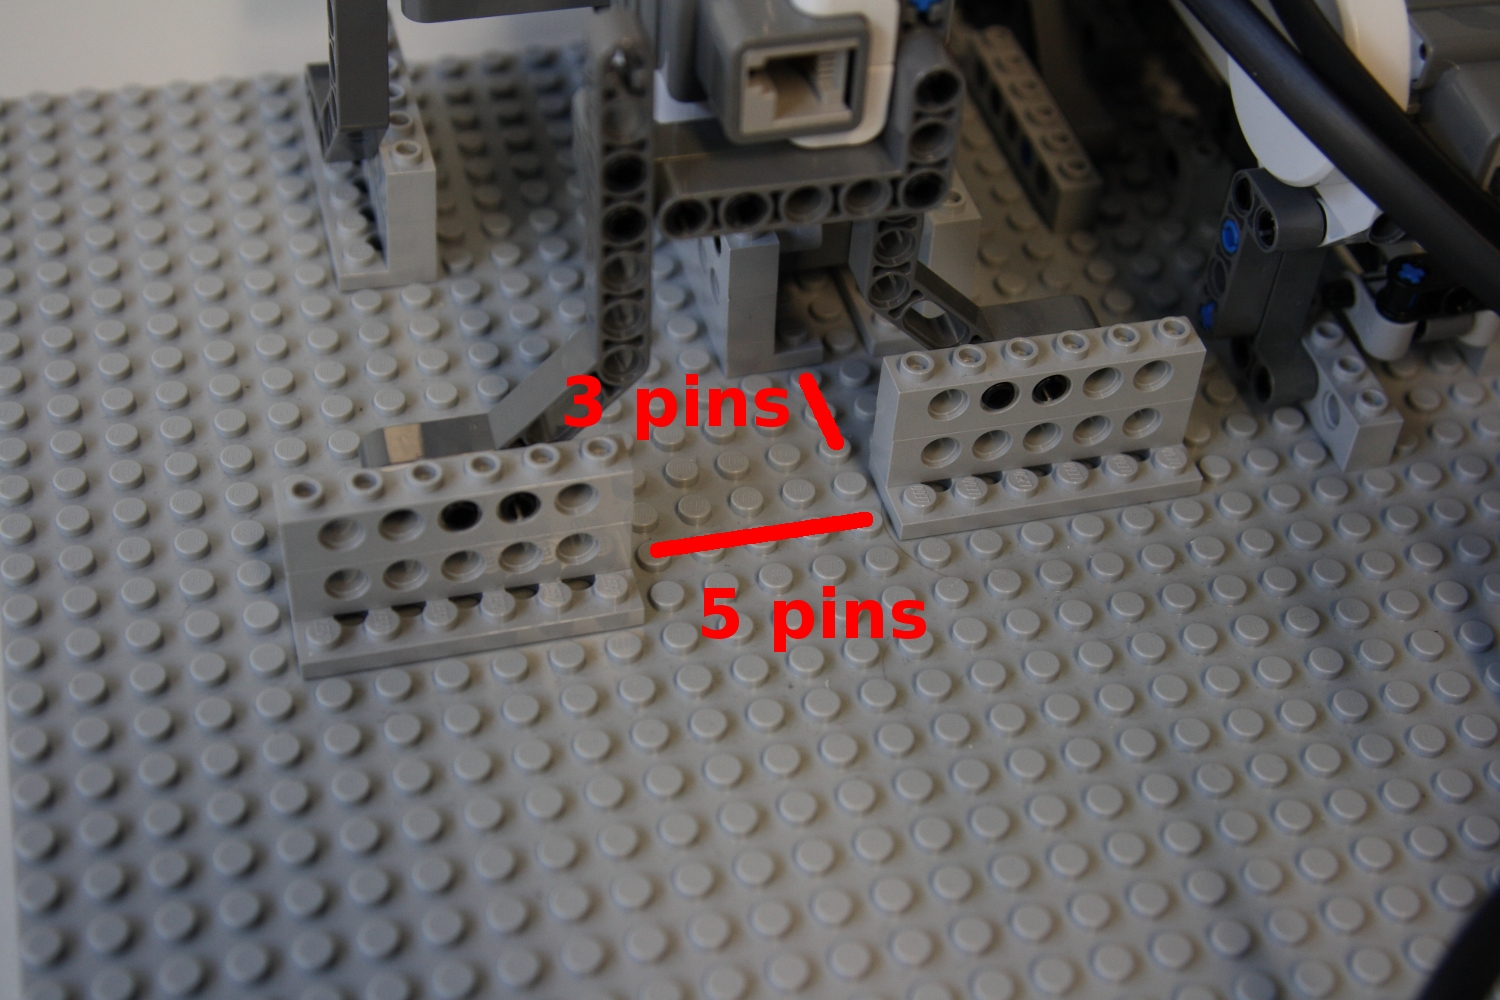
\includegraphics[scale=0.3]{graphics/4.jpg}
\end{center}
\caption{Image taken from position 4}
\label{pic:position4}
\end{figure}

\newpage

\subsection{The supporting bridge at the end of the tape}

Figure \ref{pic:bridge2} shows how the upper piers of the supporting bridge have to be placed in relation to the lower and right edge of the upper plate.

\begin{figure}[!htb]
\begin{center}
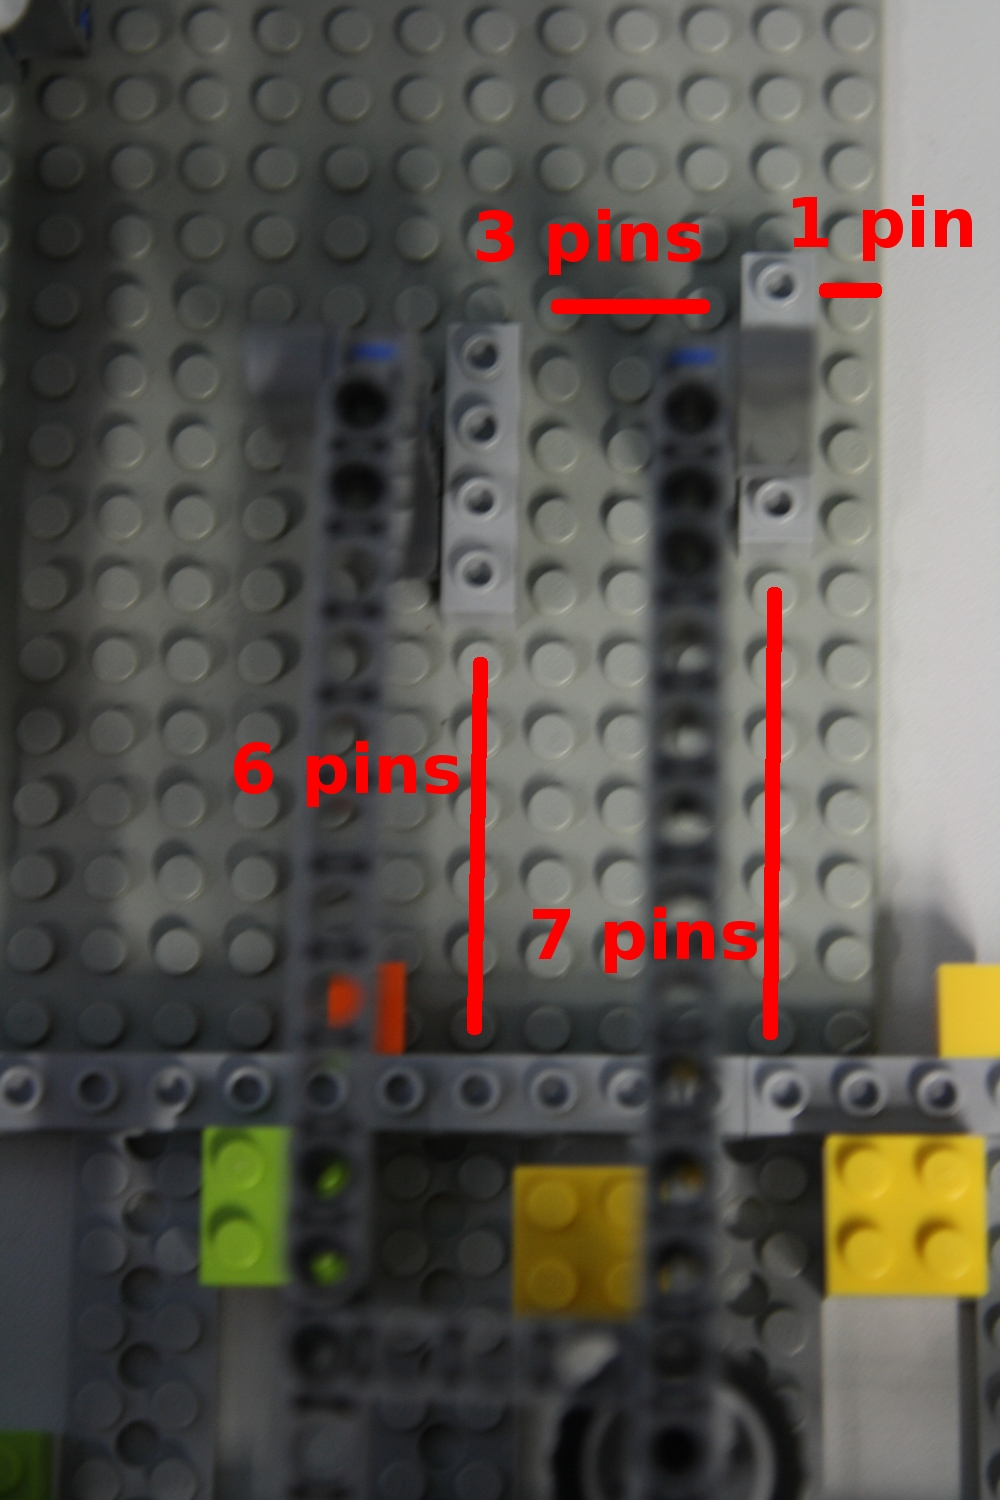
\includegraphics[scale=0.35]{graphics/bridge2.jpg}
\end{center}
\caption{Position of the bridge}
\label{pic:bridge2}
\end{figure}

\newpage

Figure \ref{pic:bridge1} shows how the lower piers of the supporting bridge have to be placed in relation to the upper and right edge of the lower plate.

\begin{figure}[!htb]
\begin{center}
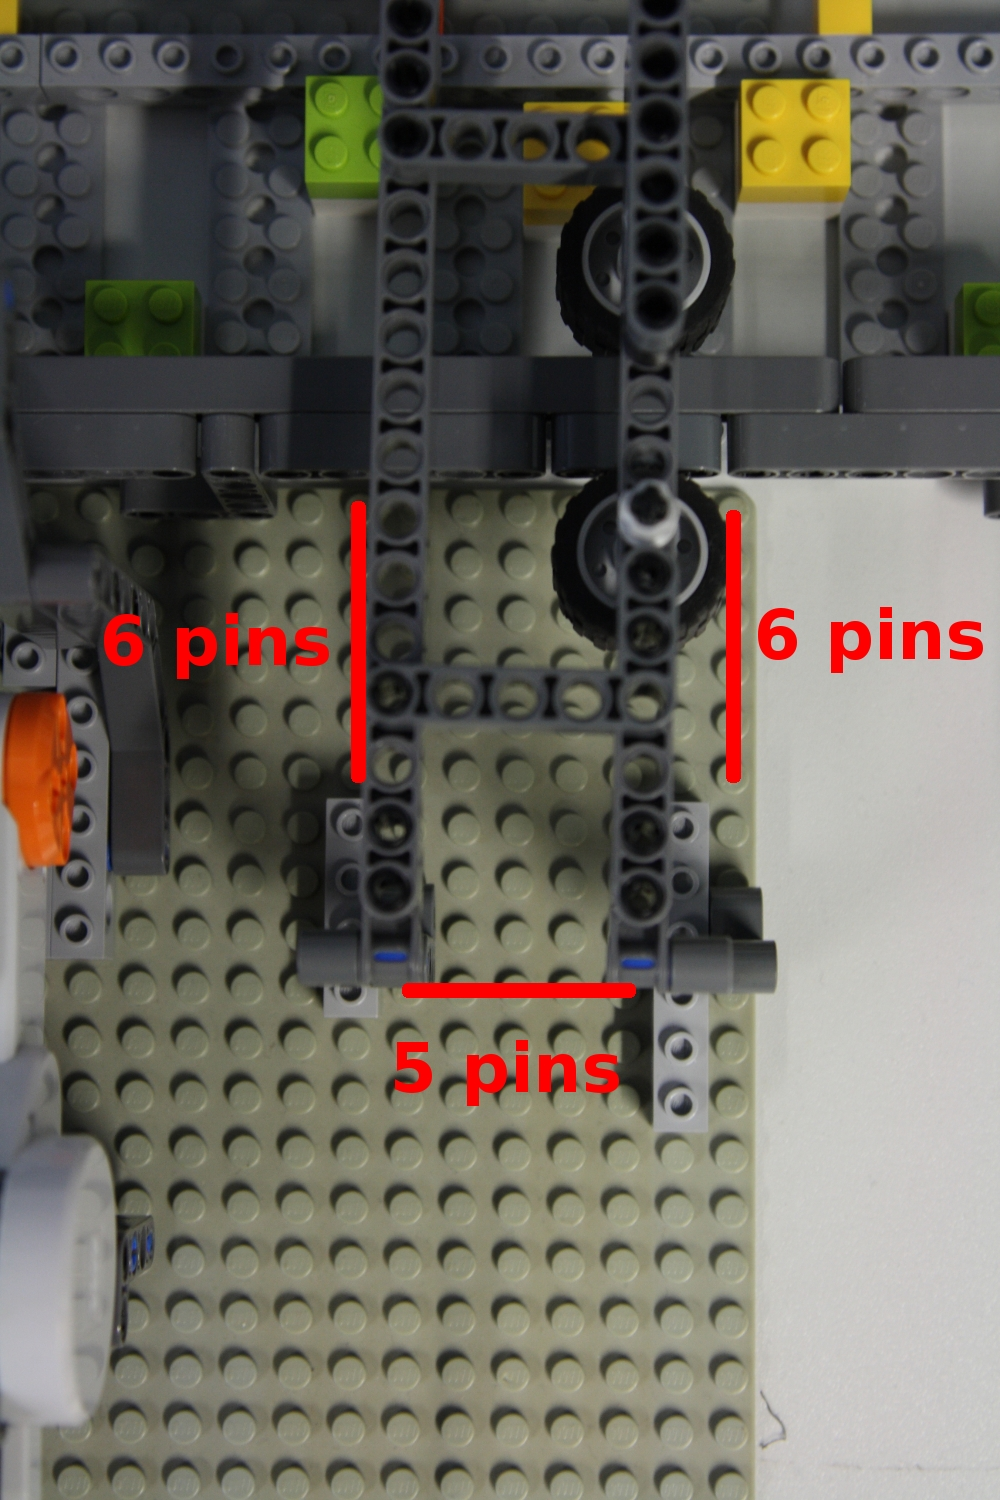
\includegraphics[scale=0.35]{graphics/bridge1.jpg}
\end{center}
\caption{Position of the bridge}
\label{pic:bridge1}
\end{figure}

\newpage

\subsection{The sensors}

Figure \ref{pic:sensors} shows how the sensors have to be placed to work properly. As you can see the sensor it the rectangle 1 has to be above one of the position bits every time the sensors in rectangle 2 are above two bits at one of the positions.

\begin{figure}[!htb]
\begin{center}
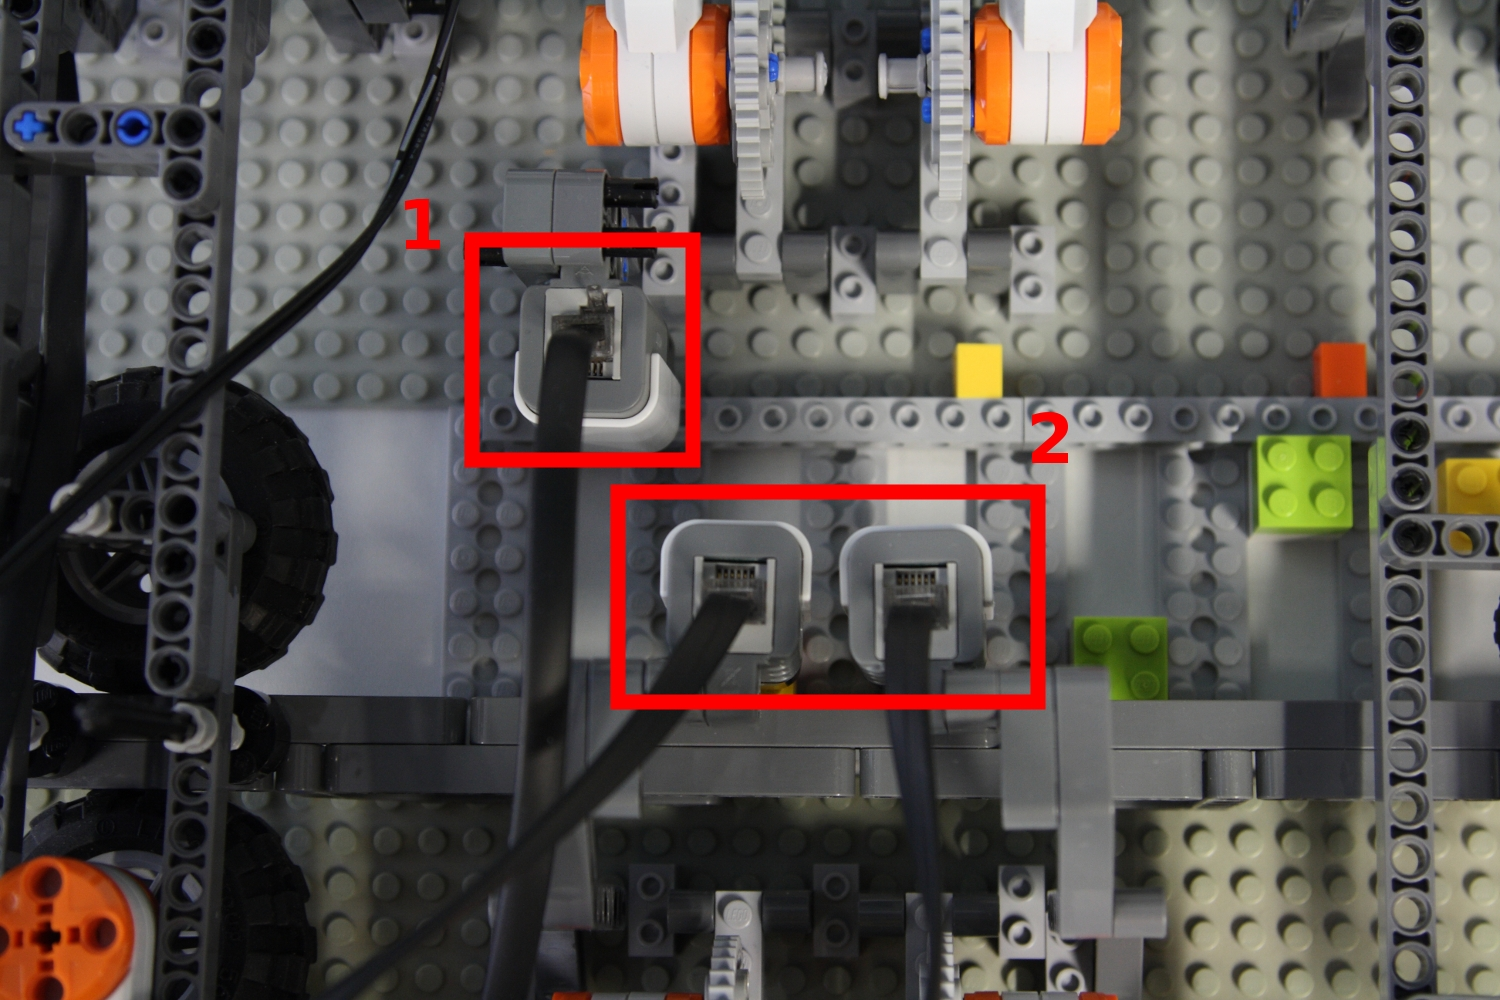
\includegraphics[scale=0.3]{graphics/sensors.jpg}
\end{center}
\caption{Position of the sensors}
\label{pic:sensors}
\end{figure}

\newpage

\subsection{The tape}

The Marker in Figure \ref{pic:tape} shows how the bricks have to be placed so the sensors recognize them and can distinguish the different positions of the tape. It is also very important that the piers used for the upper bar of the tape are not interfering with the pushers shown in Figure \ref{pic:topview_pushers} and Figure \ref{pic:pusher}. So the pier you can see in the background of Figure \ref{pic:tape} is placed perfectly because it is not preventing the pushers from moving the bits.

\begin{figure}[!htb]
\begin{center}
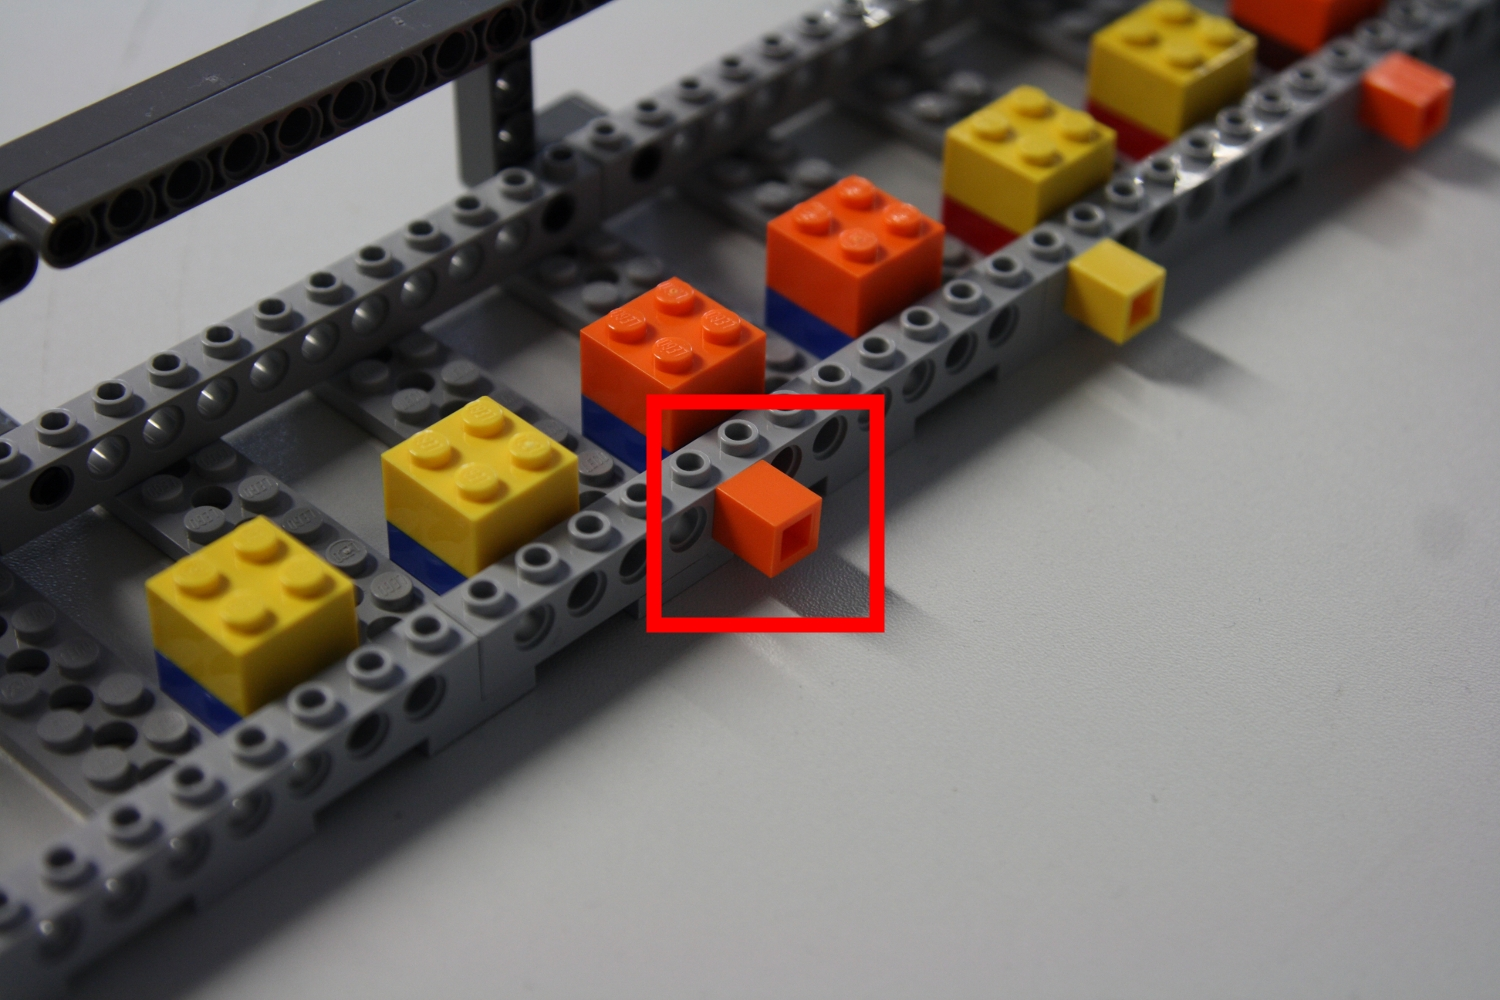
\includegraphics[scale=0.3]{graphics/tape.jpg}
\end{center}
\caption{The tape}
\label{pic:tape}
\end{figure}

\newpage

Figure \ref{pic:supporting_pier} shows how the supporting piers have to be placed so they do not interfere with the pushers. It also shows how the sensors in the rectangle 2 in figure \ref{pic:sensors} have to be placed so they are above the bits every time the sensor in rectangle 1 is above a position bit.

\begin{figure}[!htb]
\begin{center}
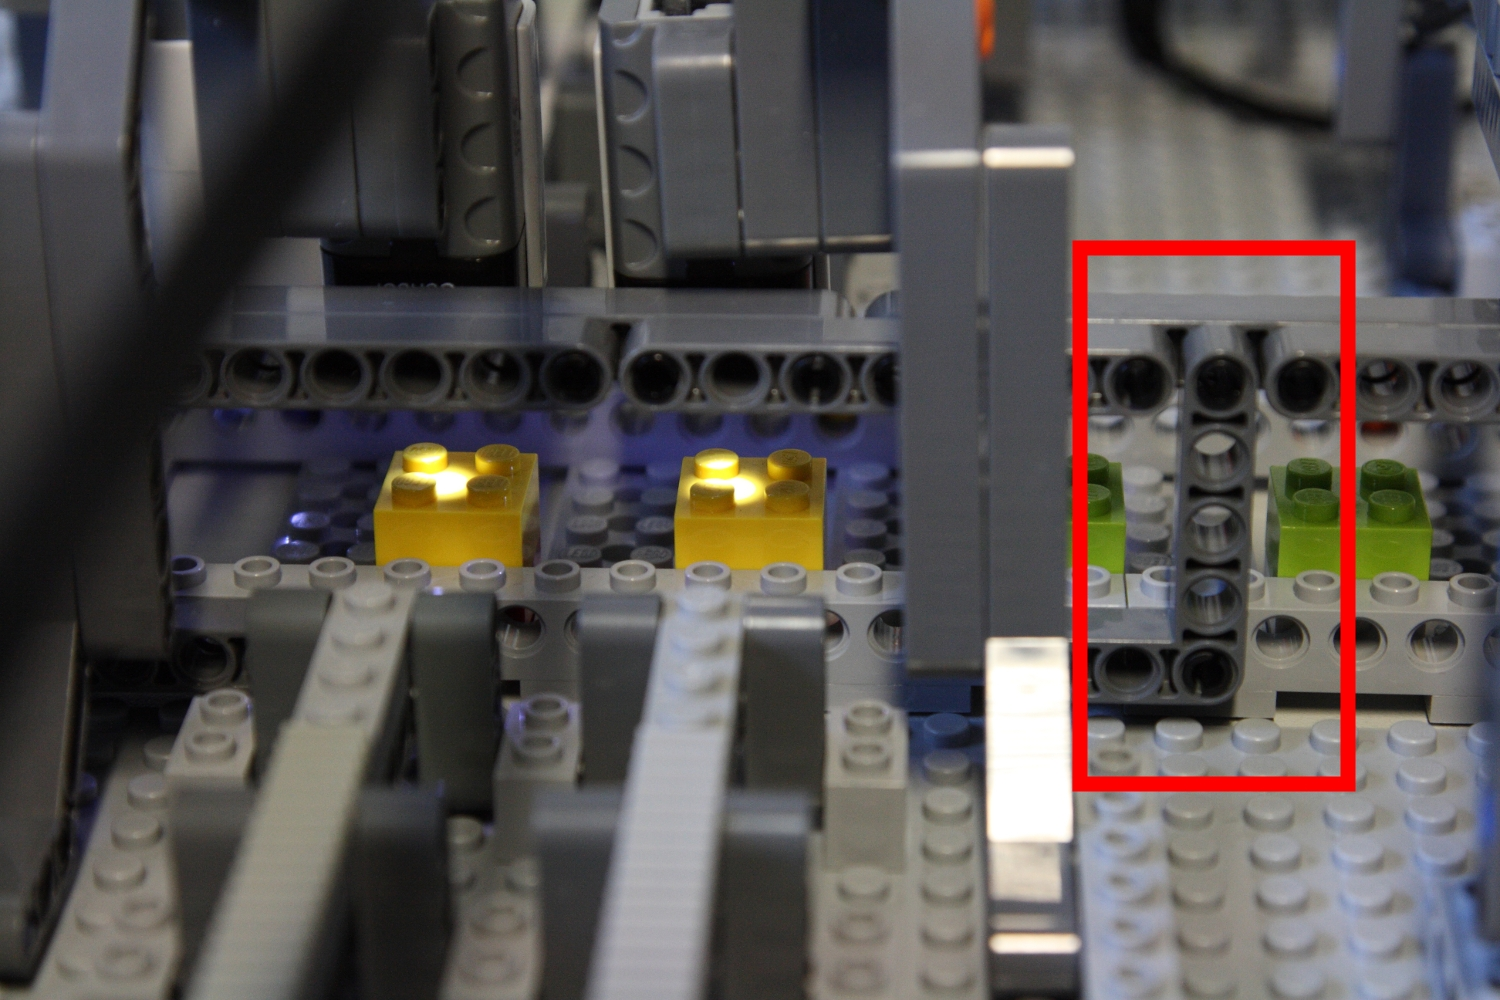
\includegraphics[scale=0.3]{graphics/supporting_pier.jpg}
\end{center}
\caption{One of the supporting piers}
\label{pic:supporting_pier}
\end{figure}

\newpage

\subsection{The pushers}

Figure \ref{pic:pusher} shows how the pushers have to be placed on the guard rail so they can be pushed properly by the gear wheels.

\begin{figure}[!htb]
\begin{center}
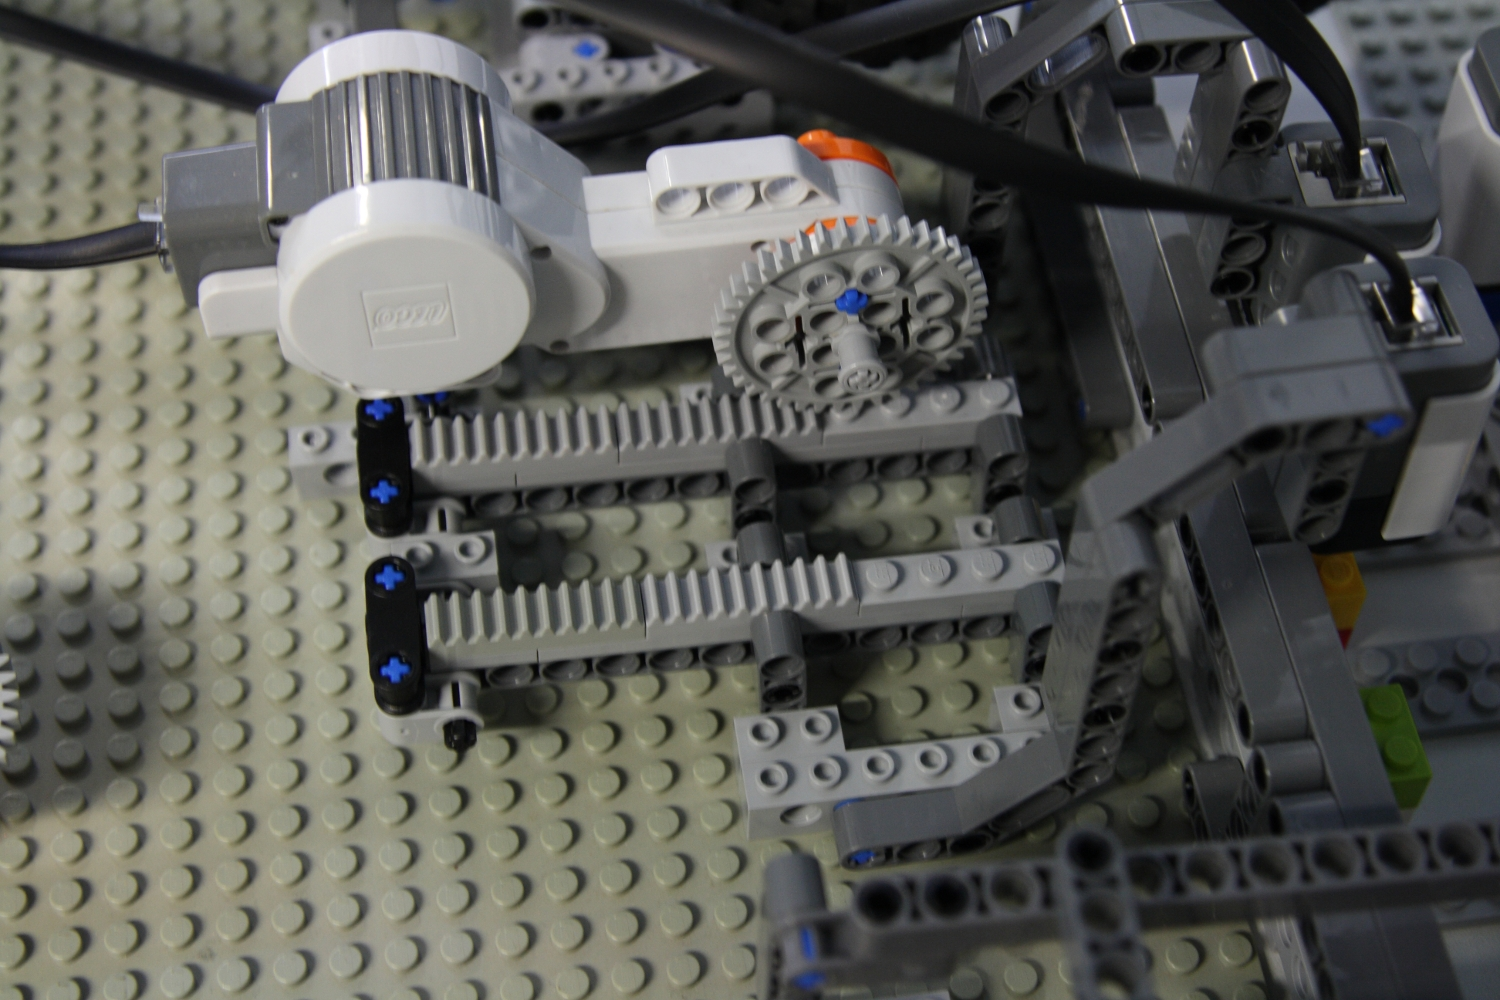
\includegraphics[scale=0.3]{graphics/pusher.jpg}
\end{center}
\caption{Pusher}
\label{pic:pusher}
\end{figure}

\newpage

Figure \ref{pic:topview_pushers} shows how the pushers are pushing the bits and how to place the supporting piers (rectangle) for the tape's upper bar so they do not interfere with the pushers.

\begin{figure}[!htb]
\begin{center}
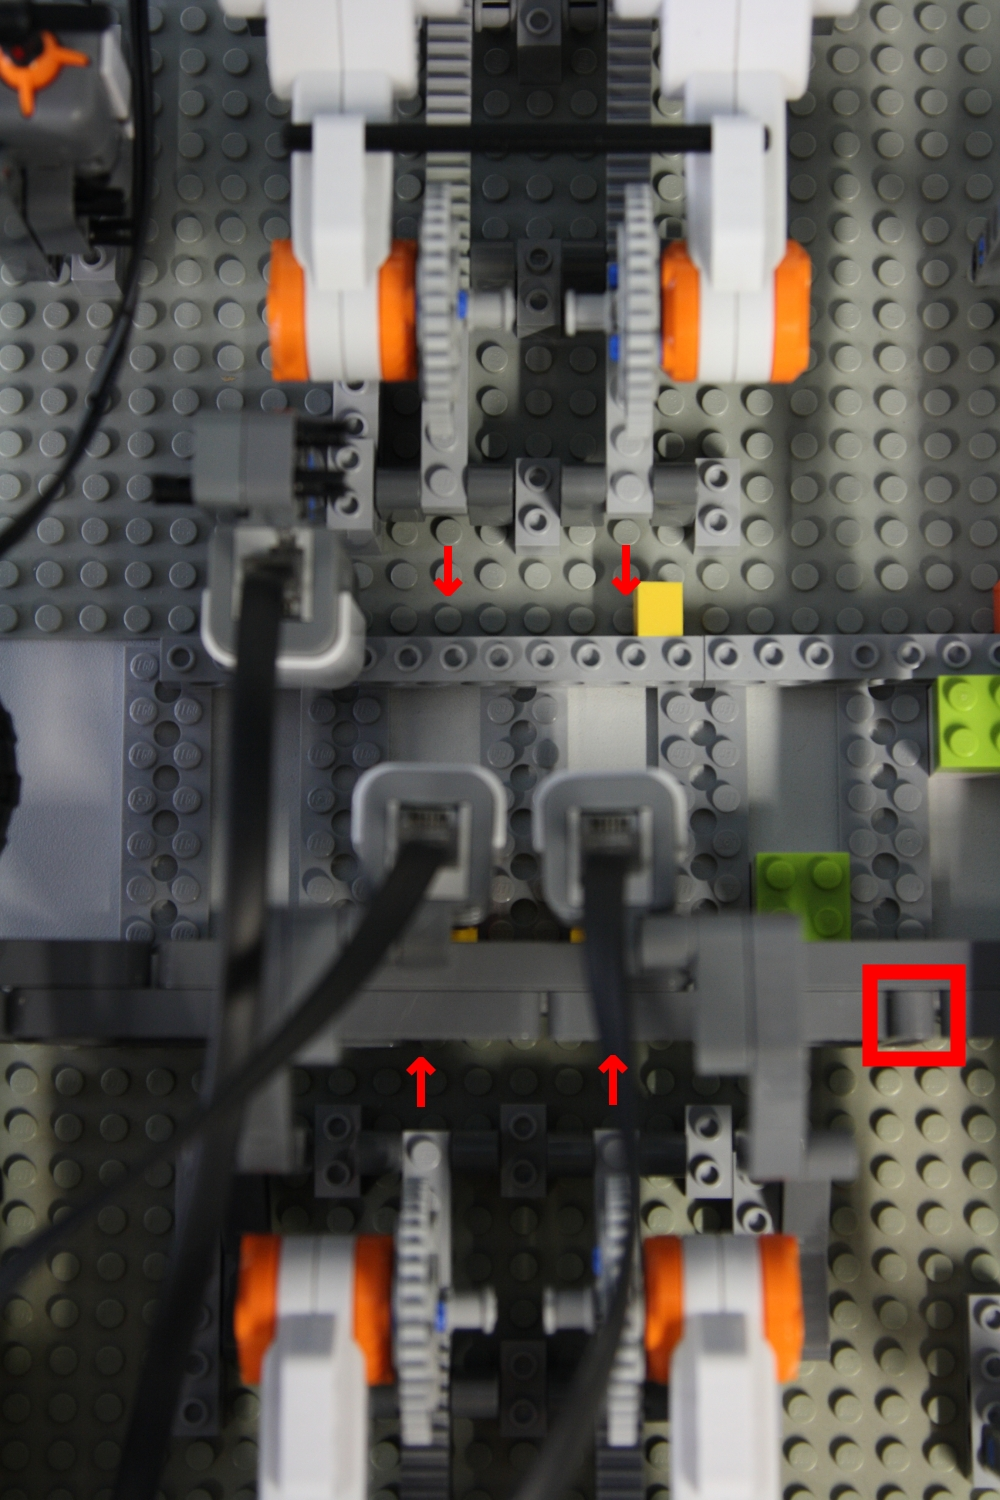
\includegraphics[scale=0.35]{graphics/topview_pushers.jpg}
\end{center}
\caption{Position of the pushers}
\label{pic:topview_pushers}
\end{figure}

\makebackpage[trisec]%[<plain/info/addressinfo>]

\end{document}
